\documentclass{article}
\usepackage[ngerman]{babel}
\usepackage[utf8]{inputenc}
\usepackage{graphicx} 
\usepackage{svg}
\usepackage{booktabs}
\usepackage{longtable, lscape}
\usepackage{tikz}
\usepackage{multicol}
\usepackage{longtable}
\usepackage{array} 
\usepackage{varwidth}
\graphicspath{{img/}}
\usepackage{geometry}
\usepackage{amsmath}
\usepackage{pdflscape}
\geometry{a4paper, top=25mm, left=30mm, right=25mm, bottom=20mm}

\begin{document}

\section{Einführung}

Messungen:
\begin{itemize}
\item Beschleunigung Sensor1 und Sensor2 bei 45 Grad
\item Beschleunigung Sensor1 und Sensor2 bei 30 Grad
\item Beschleunigung Sensor1 und Sensor2 bei 15 Grad
\item Beschleunigung Sensor1 und Sensor2 bei 0  Grad
\item Beschleunigung Sensor1 und Sensor2 bei -15 Grad
\item Beschleunigung Sensor1 und Sensor2 bei -30 Grad
\item Beschleunigung Sensor1 und Sensor2 bei -45 Grad
\item Winkelgeschwindigkeit Sensor1 und Sensor2 bei 0 rad/sec
\end{itemize}

\section{Aktorik und Sensorik}
Der folgenden Abschnitt beschreibt die verwendeten elektrischen Bauteile, um einerseits die benötigten physikalischen Größen zu messen, und andererseits die verwendete Aktorik, um das Aufspringen und Balancieren der Würfelseite zu ermöglichen.
\newline 

Die Aufgabe der Sensorik besteht darin die Zustandsgrößen des Systemes zu bestimmen. Hierfür werden zwei \textit{GYR-521}-Platinen verwendet, die mit einem \textit{MPU6050}-IC der Firma \textit{InvenSense} bestückt sind. Diese bieten jeweils einen dreiachsigen Beschleunigungssensor und Gyroskop. Mit Hilfe dieser Messwerte können die Zustandsgrößen $\varphi$ und $\dot{\varphi}$ berechnet werden. Die Sensoren bieten die zusätzliche Möglichkeit einen variablen Tiefpassfilter zu verwenden um eine erste Glättung der Messwerte durchzuführen. Dieser Tiefpassfilter wird auf eine Grenzfrequenz von $44Hz$ eingestellt. Dieser Wert hat sich empirisch als optimaler Kompromiss zwischen Filterung der Rauschsignale und Verzögerung des eigentlichen Signals. Die Konfiguration und Auswertung der Sensoren erfolgt über eine $I^2C$-Schnittstelle. Die Justierung und Auswertung der Sensoren wird näher in \ref{sensorik_sec} beschrieben.
\newline

Abschnitt \ref{Dynamik_sec} zeigt den Einfluss eines Motormomentes auf die Position und Gewschwindigkeit der Würfelseite. Um diese Moment zu erzeugen wird ein bürstenloser DC-Motor der Firma \textit{MaxonMotor} verwendet (EC 45 flat, 50 Watt). Die Kriterien zur Auswahl des Motors sind einerseits die maximale Drehzahl und Drehmoment, andererseits die mechanische Zeitkonstante. Für das Aufspringen des Würfels ist die maximale Drehzahl des Motors von Bedeutung, die 10000 Umdrehung pro Minute des gewählten Motor reichen hierbei aus um eine ausreichend hohe kinetische Energie der Schwungmasse zu ermöglichen. Die Robustheit der Regelung wird durch das maximale Drehmoment limitiert, welches in diesem Fall bei 83.4 mNm liegt. Von besondere Bedeutung für die Regelung ist die mechanische Zeitkonstante des Motors, da diese eine Verzögerung der Stellgröße bewirkt und somit den geschlossenen Regelkreis negativ beeinflussen kann. Die mechanische Zeitkonstante des gewählten Motors ist mit $13.3ms$ im Vergleich zu anderen Kandidaten sehr niedrig. Die Ansteuerung des Motors erfolgt über den Treiberbaustein \textit{ESCON 36/3 EC}, welcher ebenfalls von der Firma \textit{Maxon Motor} vertrieben wird. Dieser ermöglicht die Steuerung des Drehmoments über ein PWM-Signal und die Auswertung der Winkelgeschwindigkeit $\dot{\psi}$ über ein analoges Signal.
\newline

Mit Hilfe einer mechanischen Bremse kann die Schwungmasse stoßartig zum Stillstand gebracht werden. Dadurch wird die kinetische Energie der Schwungmasse teilweise auf das Gesamtsystem übertragen und ermöglicht somit das Aufspringen. Die Bremsbacken werden über einen Servomotor betätigt, welcher mit Hilfe eines PWM-Signales kontrolliert wird.
\newline

Zur Ansteuerung der Aktorik und Sensorik wird ein STM32F4Discovery-Board der Firma \textit{STMicroelectronics} verwendet. Die Programmierung erfolgt über eine, auf Eclipse basierende, Toolkette. Um die Auswertung der Sensordaten und den Entwurf der Regelung zu erleichtern, wird der Quellcode anschließend in Simulink-Blöcke implementiert.


\section{Modellierung der Systemdynamik} \label{Dynamik_sec}
In dem folgenden Abschnitt werden die Bewegungsgleichungen mit Hilfe des Lagrange Formalismus hergeleitet. Aus diesen Gleichung kann im Anschluss eine Zustandsraumdarstellung aufgestellt werden, welche als Grundlage für den Reglerentwurf dient.

\begin{figure}[h]
\centering
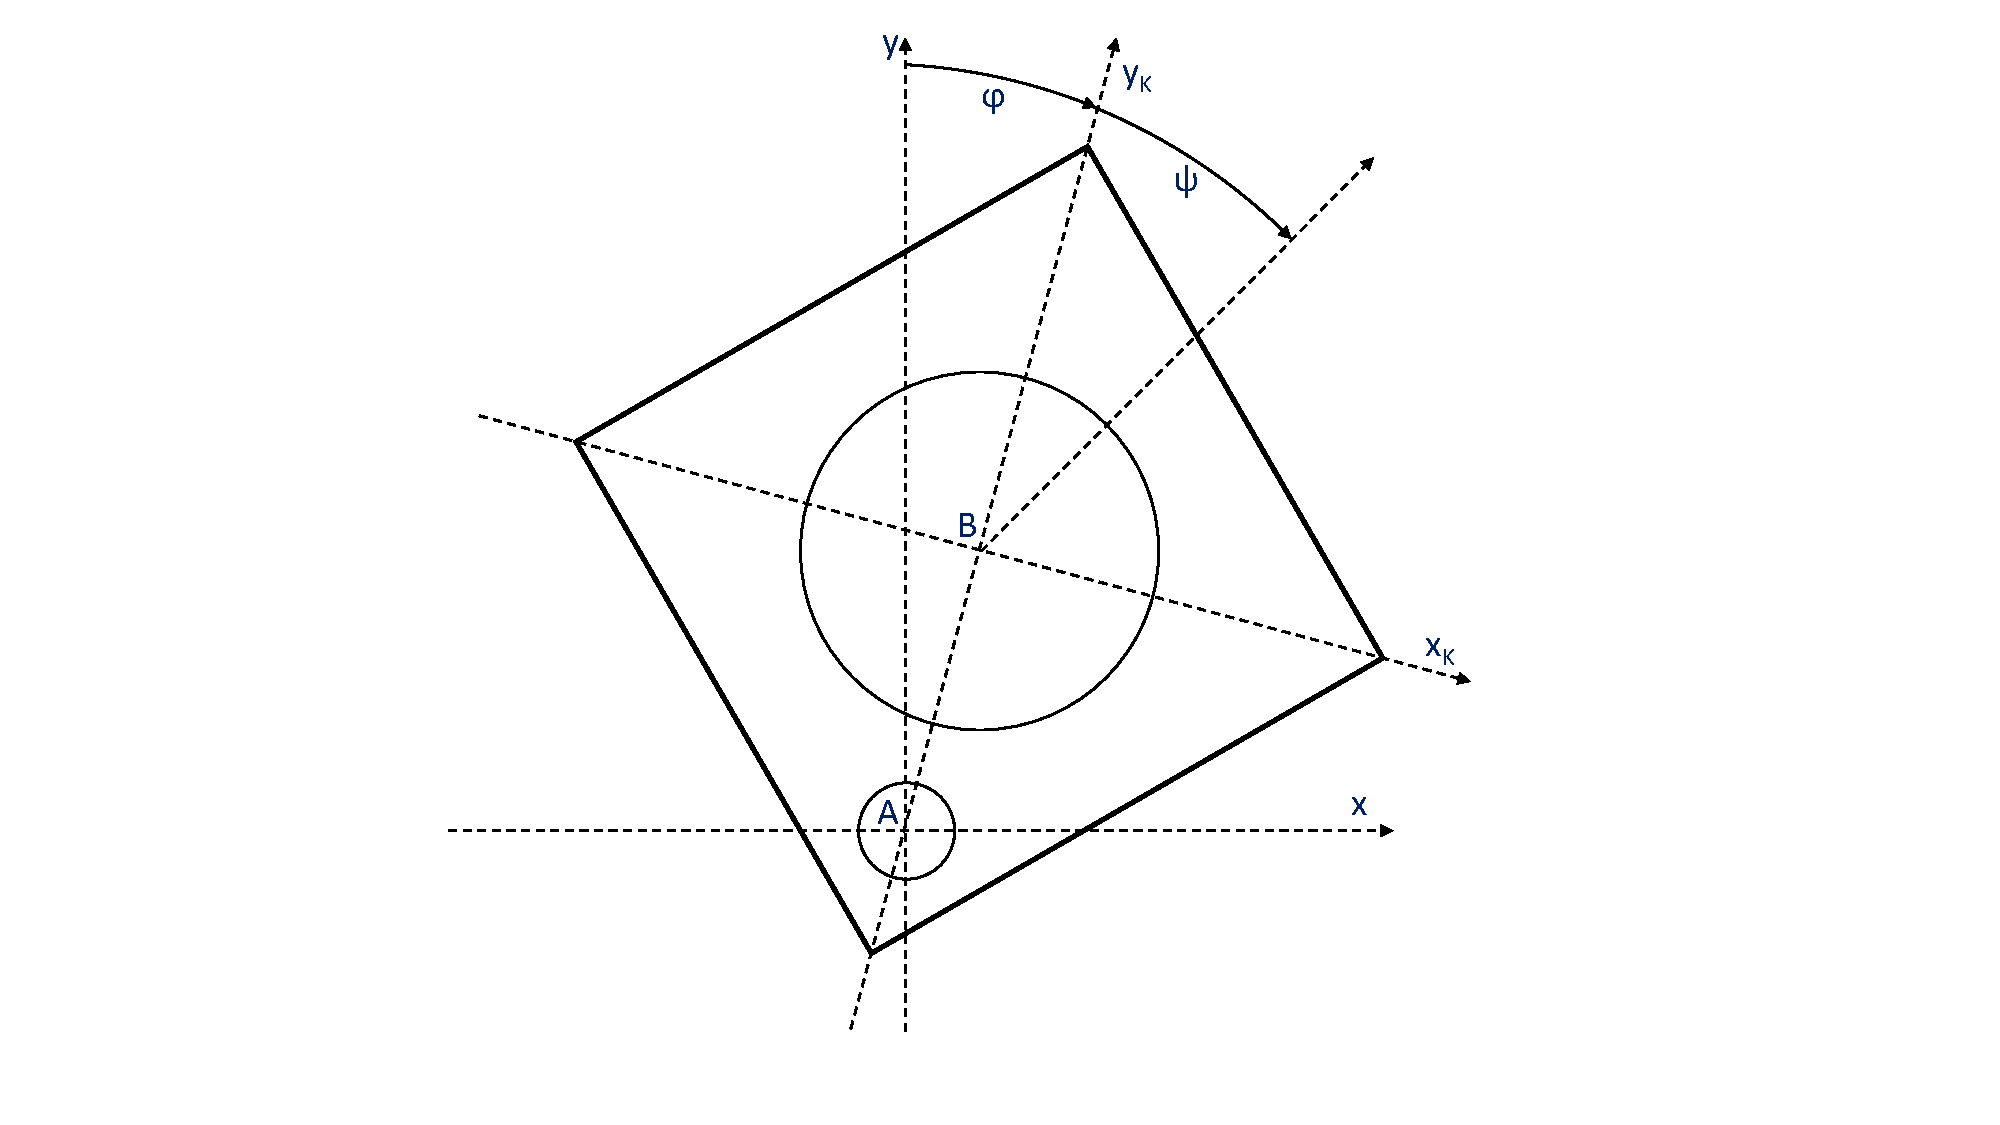
\includegraphics[width=\linewidth]{MechZeichnung1D}
\caption{Mechanischer Aufbau, Quelle: eigene Darstellung}
\end{figure}

Der Prototyp besteht aus einem starren Körper der in $A$ auf einer Achse gelagert ist. In $B$ ist eine Schwungmasse über einen Motor mit dem Körper verbunden. Somit verfügt das Gesamtsystem über zwei Freiheitsgrade, welche durch die generalisierten Koordinaten 

\begin{equation}
q_1 = \varphi \hspace{35pt} q_2 = \psi
\end{equation}

beschrieben werden. Der Winkel $\varphi$ wird von den Achsen $y$ und $y_K$ eingeschlossen. Der Winkel beschreibt die rotatorische Verschiebung der Schwungmasse zu dem Körper. Die folgenden Größen beschreiben die weiteren physikalischen Gegebenheiten des Systems.\newline

\begin{table}[h]
\centering
\begin{tabular}{|c|c|}
\hline
	\textbf{Variable} & \textbf{Erklärung} \\ \hline
	$q_1 = \varphi$ & Ausfallwinkel des Körpers \\ \hline
	$q_2 = \psi$ & Winkel zwischen Schwungmasse und Körper \\ \hline
	$A$ & Drehpunkt des Körpers \\ \hline
	$B$ & Drehpunkt des Schwungrades \\ \hline
	$l_{AB}$ & Abstand zwischen $A$ und $B$ \\ \hline
	$l_{AC}$ & Abstand zwischen $A$ und dem Schwerpunkt des Körpers \\ \hline
	$m_K$ & Masse des Körpers \\ \hline
	$m_R$ & Masse des Schwungrades \\ \hline
	${\theta}^A_K$ & Massenträgheitsmoment des Körper um $A$ \\ \hline
	${\theta}^B_R$ & Massenträgheitsmoment der Schwungmasse um $B$ \\ \hline
	$C_{\varphi}$ & Dynamischer Reibkoeffizient des Körpers in $A$ \\ \hline
	$C_{\psi}$ & Dynamischer Reibkoeffizient des Schwungrades in $B$ \\ \hline
	$T_M$ & Drehmoment des Motor \\ \hline
\end{tabular}
\end{table}

\newpage
Um die Bewegungsgleichungen des Systems zu ermitteln wird der Lagrange Formalismus verwendet. Dieser basiert auf der Lagrange-Funktion $L$, welche die Differenz der kinetischen Energie $T$ und der potenziellen Energie $V$ des Systems beschreibt.

\begin{equation}
T = \frac{1}{2}[({\theta}^A_K + m_R \cdot {l_{AB}}^2) {\dot{\varphi}}^2 + {\theta}^R_B(\dot{\varphi}+\dot{\psi})^2]
\end{equation}
\begin{equation}
V = g(m_R \cdot l_{AB} + m_K \cdot l_{AC})cos(\varphi)
\end{equation}
\begin{equation}
L = T - V = \frac{1}{2}[({\theta}^A_K + m_R \cdot {l_{AB}}^2) {\dot{\varphi}}^2 + {\theta}^R_B(\dot{\varphi}+\dot{\psi})^2] - g(m_R \cdot l_{AB} + m_K \cdot l_{AC})cos(\varphi)
\end{equation}

In dem System wirken unterschiedliche Kräfte. Einerseits erzeugt der Motor ein Drehmoment, welches die virtuelle Arbeite $\delta W_M$ verursacht. Andererseits verrichtet die Gravitation die virtuelle Arbeite $\delta W_G$. Zusätzlich muss die, durch die Reibung entstandene, Verlustleistung berücksichtigt werden. In diesem Fall wird die Reibleistung mit den Rayleigh'schen Dissipationsfunktionen $D_{\varphi}$ und $D_{\psi}$ beschrieben und verrichten die virtuelle Arbeit $\delta W_D$.

\begin{equation}
-\delta W_M = T_M \cdot \delta \psi
\end{equation}

\begin{equation}
-\delta W_G = g(m_K \cdot l_{AC} + m_R \cdot l_{AB})sin(\varphi) \cdot \delta \varphi
\end{equation}

\begin{equation}
D_{\varphi} = \frac{1}{2}C_{\varphi} \cdot {\dot{\varphi}}^2
\end{equation}
\begin{equation}
D_{\psi} = \frac{1}{2}C_{\psi} \cdot {\dot{\psi}}^2
\end{equation}
\begin{equation}
D = D_{\varphi} + D_{\psi} = \frac{1}{2}C_{\varphi} \cdot {\dot{\varphi}}^2 + \frac{1}{2}C_{\psi} \cdot {\dot{\psi}}^2
\end{equation}
\begin{equation}
-\delta W_D = - C_{\varphi} \cdot \dot{\varphi} \cdot \delta \varphi - C_{\psi} \cdot \dot{\psi} \cdot \delta \psi
\end{equation}

Die Summe der virtuellen Arbeiten, welche von den verschiedenen Kräften verrichtet wird, ergibt die virtuelle Arbeit des Gesamtsystems $\delta W$. In dem die verrichtete Arbeit partiell nach den beiden generalisierten Koordinaten $\varphi$ und $\psi$ differenziert wird, können die beiden generalisierten Kraftkomponenten $Q_{\varphi}$ und $Q_{\psi}$ berechnet werden.

\begin{equation}
Q_{\varphi} = g(m_K \cdot l_{AC} + m_R \cdot l_{AB})sin(\varphi) - C_{\varphi} \cdot \dot{\varphi}
\end{equation}
\begin{equation}
Q_{\psi} = T_M - C_{\psi} \cdot \dot{\psi}
\end{equation}


Bei dem Prototyp handelt es sich um ein nicht konservatives System, da durch die Reibung mechanische Energie verloren geht und der Motor dem System mechanische Energie zuführt. Da die beiden generalisierten Koordinaten $\varphi$ und $\psi$ voneinander unabhängig sind können aus dem d'Alembert'schen Prinzip zwei Bewegungsgleichungen abgeleitet werden.

\begin{equation}
\frac{d}{dt}\frac{\partial T}{\partial \dot{q}_i}-\frac{\partial T}{\partial q_i} = Q_i
\end{equation}
\begin{equation}
\frac{d}{dt}\frac{\partial T}{\partial \dot{\varphi}}-\frac{\partial T}{\partial \varphi} = Q_{\varphi} 
\end{equation}
\begin{equation}
\label{LG_phi_equation}
({\theta}^A_K + {\theta}^B_R + m_R \cdot l_{AB}^2)\ddot{\varphi} + {\theta}^B_R \cdot \ddot{\psi} - g(m_R \cdot l_{AB} + m_K \cdot l_{AC})sin(\varphi) + C_{\psi} \cdot \dot{\psi} = 0
\end{equation}
\begin{equation}
\frac{d}{dt}\frac{\partial T}{\partial \dot{\psi}}-\frac{\partial T}{\partial \psi} + \frac{\partial T}{\partial \dot{\psi}} = Q_{\psi} 
\end{equation}
\begin{equation}
\label{LG_psi_euqation}
{\theta}^R_B \cdot \ddot{\psi} = T_M - C_{\psi} \cdot \dot{\psi} - {\theta}^B_R \cdot \ddot{\varphi}
\end{equation}

Durch Einsetzen von (\ref{LG_psi_euqation}) in (\ref{LG_phi_equation}) ergibt sich die folgende Bewegungsgleichung für die Würfelseite.

\begin{equation}
\label{BG_phi_quation}
\ddot{\varphi} = \frac{g(m_R \cdot l_{AB}^2 + m_K \cdot l_{AC})sin(\varphi) - C_{\varphi} \cdot \dot{\varphi} + C_{\psi} \cdot \dot{\psi} - T_M}{{\theta}^A_K + m_R \cdot l_{AB}^2}
\end{equation}

Die Bewegungsgleichung für die Schwungmasse ergibt sich durch Einsetzen von (\ref{BG_phi_quation}) in (\ref{LG_psi_euqation}).

\begin{equation}
\label{BG_psi_equation}
\ddot{\psi} = \frac{({\theta}^A_K + m_R \cdot l_{AB}^2 + {\theta}^B_R)(T_M - C_{\psi} \cdot \dot{\psi})}{({\theta}^A_K + m_R \cdot {l_{AB}}^2){\theta}^B_R} + \frac{C_{\varphi} \cdot \dot{\varphi} - g(m_R \cdot l_{AB} + m_K \cdot l_{AC})sin(\varphi)}{{\theta}^A_K + m_R \cdot {l_{AB}}^2}
\end{equation}

\section{Sensorik}
\label{Sensorik_secd}
Die Aufgabe der verwendeten Sensorik liegt darin die Werte für $\varphi$, und $\dot{\varphi}$ zu bestimmen. Hierfür wurden zwei MPU6050 IC's verwendet. Diese verfügen jeweils über einen Beschleunigungssensor und Gyroskop, welche Werte für drei Achsen ausgeben. Der Tiefpass der Sensoren wird auf eine Grenzfrequenz von $44Hz$ eingestellt, da hier einerseits eine erste Glättung der Daten erfolgt, andererseits aber keine zu große Verzögerung ergibt, welche sich wiederum negativ auf die Regelung auswirken könnte. Die Position und Ausrichtung der Sensoren ist in \ref{Position_Sensoren_pic} dargestellt.

\begin{figure}[h]
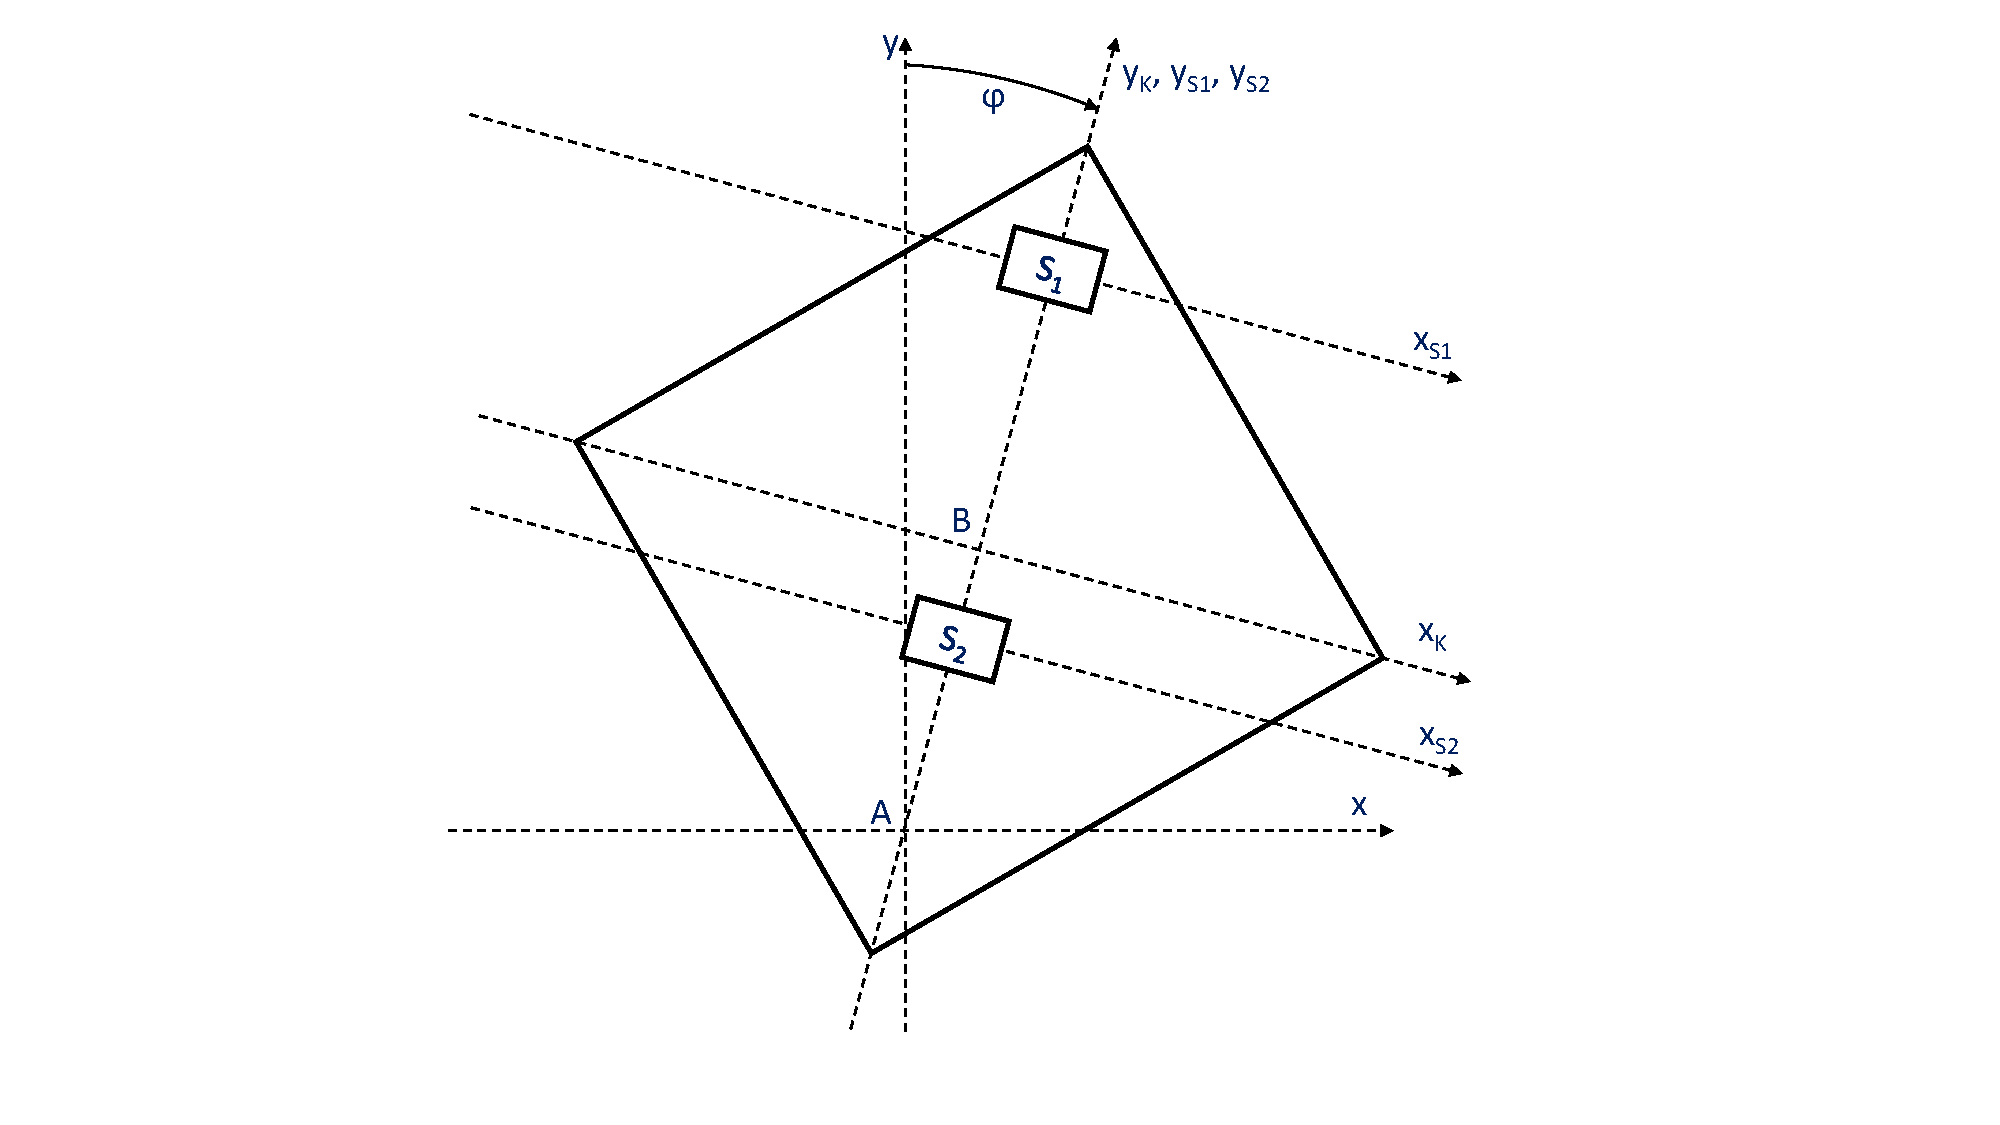
\includegraphics[width=\linewidth]{SensorZeichnung1D}
\caption{Position der Sensoren, Quelle: eigene Darstellung}

\label{Position_Sensoren_pic}
\end{figure}

\subsection{Winkelschätzung}
Die Sensoren keine Wege bzw. Winkel. Somit muss der Winkel $\varphi$ berechnet werden. Die gemessenen Sensorwerte hängen von $r_{S1}$ bzw. $r_{S2}$ ab, welche den Abstand zwischen den Sensoren und dem Drehpunkt $A$ beschreiben. Zusätzlich beeinflussen neben dem Winkel $\varphi$ auch dessen beiden Ableitungen $\dot{\varphi}$ und $\ddot{\varphi}$ die Sensorausgabe. Allerdings lassen sich aus den Beschleunigungswerten der beiden Sensoren nach \cite{Cubli1D} wie folgt der aktuelle Wert von $\varphi$ berechnen.

\begin{equation}
\ddot{S}_i = 
\begin{pmatrix}
\ddot{x}_i \\ \ddot{y}_i \\ \ddot{z}_i
\end{pmatrix} =
\begin{pmatrix}
r_{Si} \cdot \ddot{\varphi} + sin(\varphi) \cdot g \\
- r_{Si} \cdot \dot{\varphi}^2 - cos(\varphi) \cdot g \\
0
\end{pmatrix}
\hspace{35pt}
i \in [1;2]
\end{equation}

\begin{equation}
\alpha = \frac{r_{S1}}{r_{S2}}
\end{equation}

\begin{equation}
\ddot{x}_1 - \alpha \cdot \ddot{x}_2 = 
g(1 - \alpha)sin(\varphi)
\end{equation}
\begin{equation}
\ddot{y}_1 - \alpha \cdot \ddot{y}_2 = 
-g(1- \alpha)cos(\varphi)
\end{equation}

\begin{equation}
\frac{\ddot{x}_1 - \alpha \cdot \ddot{x}_2}{\ddot{y}_1 - \alpha \cdot \ddot{y}_2} = -tan(\varphi)
\end{equation}

\subsection{Kalibrierung und Justierung}
Die Sensoren geben die Beschleunigungs- und Geschwindigkeitswerte als 16 Bit Werte im Zweierkomplement aus. Diese Rohwerte müssen in die mit Hilfe eines Ausgleichspolynoms in die jeweilige SI-Einheit umgerechnet werden. 

\subsubsection{Umrechnung der Winkelgeschwindigkeiten}
In der Ruhelage werden 10000 Geschwindigkeitswerte der Sensoren aufgenommen. Über die Abweichung des Mittelwerts zu dem Sollwert ($\dot{\phi}=0$) wird die konstante Messabweichung ermittelt. Zusätzlich stellt der Hersteller einen Faktor zur Umrechnung der Roh- in SI-Werte. Daraus ergibt sich das folgende Polynom erster Ordnung zur Umrechnung der Gyroskopwerte in Winkelgeschwindigkeiten.


\subsubsection{Umrechnung der Beschleunigungswerte}
Um das Polynom zur Umrechnung der Beschleunigungswerte zu ermitteln werden sieben Messungen in den fixen Ausfallpositionen $\phi \in [-45, -30, -15, 0, 15, 30, 45]$ durchgeführt. Pro Position werden $m = 10000$ Messwerte aufgenommen. Da in der Ruhelage die Beschleunigung lediglich von dem aktuellen Ausfallwinkel abhängt ist der Sollwert für jede Position bekannt. Somit kann ein Polynom erster Ordnung approximiert werden um Mittelwerte der sieben Positionen in die entsprechenden Beschleunigungswerte umzurechnen.

%Bild mit Mittelwertvarlauf der Beschleunigungswerte x1, x2, y1, y2

\subsection{Auswertung der Radgeschwindigkeit $\dot{\psi}$}

\subsection{Filterung der Sensordaten}
In der Regel werden Sensoren von Störungen unterschiedlichster Art beeinflusst. Um diese Störungen zu minimieren werden in dem folgenden Abschnitt 


\section{Modellbildung und Bestimmung der Systemgrößen}
Mit Hilfe der Bewegungsgleichungen aus Abschnitt \ref{Dynamik_sec} kann nun eine Zustandsraumdarstellung aufgestellt werden. Hierfür werden die nichtlinearen Terme entsprechend linearisiert. Mit Hilfe der Bewegungsgleichungen bzw. Zustandsraumdarstellung kann ein Simulink-Modell implementiert werden um das Systemverhalten zu simulieren. Mit Hilfe der Zustandsraumdarstellung wird ein Zustandsregler entworfen, welcher an dem Modell erprobt werden kann. Zusätzlich über die Simulation der Einfluss der einzelnen Parameter, Sensorrauschen und Störungen untersucht werden.

\begin{equation}
\textbf{x} = \begin{pmatrix}
\varphi \\ \dot{\varphi} \\ \dot{\psi}
\end{pmatrix}
\hspace{35pt}
\textbf{y} = \begin{pmatrix}
\varphi \\ \dot{\varphi} \\ \dot{\psi}
\end{pmatrix}
\hspace{35pt}
u = T_M
\end{equation}

\begin{equation}
\dot{\textbf{x}} = \textbf{A} \cdot \textbf{x} + \textbf{B} \cdot u
\end{equation}

\begin{equation}
\textbf{y} = \textbf{C} \cdot \textbf{x} + \textbf{D} \cdot u
\end{equation}

\begin{equation}
\begin{split}
\renewcommand*{\arraystretch}{1.7}
\textbf{A} = \begin{pmatrix}
0 & 1 & 0 \\
\frac{g(m_K \cdot l_{AC} + m_R \cdot l_{AB})}{{\theta}^A_K + m_R \cdot l_{AB}^2} &
\frac{-C_{\varphi}}{{\theta}^A_K + m_R \cdot l_{AB}^2} & 
\frac{C_{\psi}}{{\theta}^A_K + m_R \cdot l_{AB}^2} \\
\frac{-g(m_K \cdot l_{AC} + m_R \cdot l_{AB)}}{{\theta}^A_K + m_R \cdot l_{AB}^2} &
\frac{C_{\varphi}}{{\theta}^A_K + m_R \cdot l_{AB}^2} &
\frac{-C_{\psi}({\theta}^A_K + {\theta}^B_R + m_R \cdot l_{AB}^2)}{{\theta}^B_R({\theta}^A_K + m_R \cdot l_{AB}^2)}
\end{pmatrix} 
\\
\renewcommand*{\arraystretch}{1.7}
\textbf{B} = \begin{pmatrix}
0 \\ \frac{-1}{{\theta}^A_K + m_R \cdot l_{AB}^2} \\ \frac{{\theta}^A_K + {\theta}^B_R + m_R \cdot l_{AB}^2}{{\theta}^K_R({\theta}^A_K + m_R \cdot l_{AB}^2}
\end{pmatrix}
\hspace{35 pt}
\textbf{C} = \begin{pmatrix}
1 & 1 & 1
\end{pmatrix}
\hspace{35pt}
\textbf{D} = \begin{pmatrix}
0
\end{pmatrix}
\end{split}
\end{equation}

\subsection{Identifikation der Parameter}
Der Reglerentwurf und die Simulation erfordern eine möglichst präzise Bestimmung der Systemparameter, wie z.B. Längen, Massen, Massenträgheitsmomente und Reibwerte. Die Bestimmung der Längen $l_{AB}$ und $l_{AC}$, der Massen $m_K$, $m_R$ und $m_G$, der Massenträgheitsmomente $\theta^A_K$ und $\theta^B_R$ erfolgt über das CAD-Modell. Hierfür werden Bauteile mit einer nicht homogenen Massenverteilung, wie z.B. die Motoren, in separate Baugruppen mit homogener Massenverteilung unterteilt.

\subsubsection{Ermittlung des Reibwertes $C_{\varphi}$}
In dem die Schwungmasse fest mit der Würfelseite verbunden wird ergibt sich die folgende Bewegungsgleichung für das Gesamtsystem.

\begin{equation}
\label{ermittlung_c_phi_equation}
(\theta^A_K + \theta^B_R + m_R  \cdot l_{AB}^2) \ddot{\varphi} = g(m_K \cdot l_{AC} + m_R \cdot l_{AB})sin(\varphi) - C_{\varphi} \cdot \dot{\varphi}
\end{equation}

In dem Versuchsaufbau wird das Gesamtsystem nun von einem Startwinkel $\varphi_0$ losgelassen, woraufhin eine gedämpfte Schwingung entsteht. Mit Hilfe der Sensoren können die Größen $\varphi$, $\dot{\varphi}$ und $\ddot{\varphi}$ gemessen werden.

\begin{figure}[h!]
\centering
 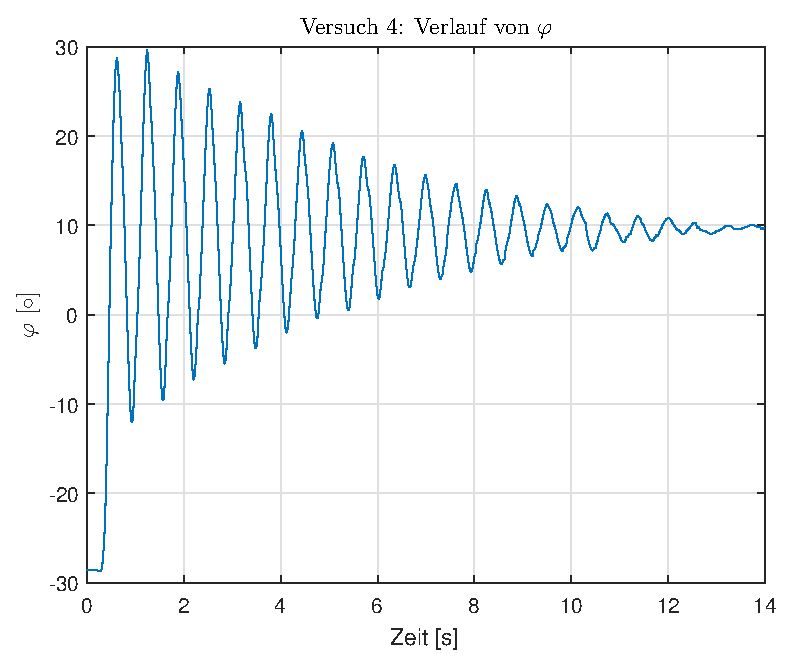
\includegraphics[width=0.5\linewidth]{img/V4_phi.eps}
	\caption{Ausfallwinkel der Würfelseite bei Versuch 4, Quelle: eigene Darstellung}
\end{figure}

Über die $n$ Messpunkte ergeben sich die folgenden Vektoren.

\begin{equation}
\boldsymbol{\varphi} = \begin{pmatrix} \varphi_1 \\ \varphi_2 \\ \vdots \\ \varphi_n \end{pmatrix} \hspace{35pt}
\boldsymbol{\dot{\varphi}} = \begin{pmatrix}
\dot{\varphi_1} \\ \dot{\varphi_2} \\ \vdots \\ \dot{\varphi_n}
\end{pmatrix} \hspace{35pt}
\boldsymbol{\ddot{\varphi}} = \begin{pmatrix}
\ddot{\varphi_1} \\ \ddot{\varphi_2} \\ \vdots \\ \ddot{\varphi_n}
\end{pmatrix}
\end{equation}

Damit ergibt sich durch Umstellen von \ref{ermittlung_c_phi_equation} die folgende Gleichung.

\begin{equation}
C_{\varphi} \cdot \boldsymbol{\dot{\varphi}} = g(m_K \cdot l_{AC} + m_R \cdot l_{AB})sin(\boldsymbol{\varphi}) - (\theta^A_K + \theta^B_R + m_R  \cdot l_{AB}^2) \boldsymbol{\ddot{\varphi}}
\end{equation}

Mit Hilfe der Methode der kleinsten Fehlerquadrate kann nun der Reibwert $C_{\varphi}$ bestimmt werden.

\begin{equation}
C_{\varphi} = 6.2 \cdot 10^{-3} \cdot kg \cdot m^2 \cdot s^{-1}
\end{equation}


\subsubsection{Ermittlung des Reibwertes $C_{\psi}$}
Im nächsten Versuchsaufbau wird die Würfelseite fixiert ($\dot{\varphi} = 0$). Hierbei beschleunigt der Motor die Schwungmasse mit einem konstanten Drehmoment $T_M=10mNm$. $T_M$ ist so zu wählen, dass sich die Radgeschwindigkeit $\dot{\psi}$ in einem Bereich bewegt, welcher dem Arbeitsbereich des geschlossenen Regelkreises entspricht. 

\begin{figure}[h!]
\centering
\includegraphics[width=0.5\linewidth]{img/V5_C_psi_d.eps}
\caption{Versuch 5: Verlauf der Radgeschwindigkeit, Quelle: eigene Darstellung}
\end{figure}


Da die Bewegung auf einen Freiheitsgrad beschränkt wurde vereinfacht sich das Modell des Systems auf die folgende Bewegungsgleichung.

\begin{equation}
\label{ermittlung_c_psi_equation}
\theta^B_R \cdot \ddot{\psi} = T_M - C_\psi \cdot \dot{\psi}
\end{equation}

Im Versuchsverlauf werden bei $n$ Stützstellen die Werte von $\psi$, $\dot{\psi}$ und $\ddot{\psi}$ gemessen. Daraus ergeben sich die folgenden Vektoren.

\begin{equation}
\label{ermittlung_c_psi_vektoren_equation}
\boldsymbol{\psi} = \begin{pmatrix} \psi_1 \\ \psi_2 \\ \vdots \\ \psi_n \end{pmatrix} \hspace{35pt}
\boldsymbol{\dot{\psi}} = \begin{pmatrix}
\dot{\psi_1} \\ \dot{\psi_2} \\ \vdots \\ \dot{\psi_n}
\end{pmatrix} \hspace{35pt}
\boldsymbol{\ddot{\psi}} = \begin{pmatrix}
\ddot{\psi_1} \\ \ddot{\psi_2} \\ \vdots \\ \ddot{\psi_n}
\end{pmatrix}
\end{equation}

Durch Einsetzen von \ref{ermittlung_c_psi_vektoren_equation} in \ref{ermittlung_c_psi_equation} kann über die Methode der kleinsten Fehlerquadrate wiederum der Reibwert $C_\psi$ bestimmt werden.

\begin{equation}
C_{\psi}= 3.1176 \cdot 10^{-5} \cdot kg \cdot m^2 \cdot s^{-1}
\end{equation}

\subsubsection{Resultate der Systemidentifikation}
An Hand der beschriebenen Versuche und Methoden wurden die folgenden Werte für die Parameter des Gesamtsystems ermittelt.

\begin{table}[h]
\centering
\begin{tabular}{|c|c|}
	\hline
	\textbf{Parameter} & \textbf{Wert} \\ \hline
	$l_{AB}$ & $0.084m$\\ \hline
	$l_{AC}$ & $0.087m$ \\ \hline
	$m_K$ & $0.221kg$ \\ \hline
	$m_R$ & $0.09kg$ \\ \hline
	${\theta}^A_K$ & $2.8 \cdot 10^{-3}kg \cdot m^2$ \\ \hline
	${\theta}^B_R$ & $1.1683 \cdot 10^{e-4} \cdot kg \cdot m^2$ \\ \hline
	$C_{\varphi}$ & $6.2 \cdot 10^{-3} \cdot kg \cdot m^2 \cdot s^{-1}$ \\ \hline
	$C_{\psi}$ & $3.1176 \cdot 10^{-5} \cdot kg \cdot m^2 \cdot s^{-1}$ \\ \hline
	$r_{S1}$ & $0.14m$ \\ \hline
	$r_{S2}$ & $0.061m$ \\ \hline
\end{tabular}
\end{table}

\newpage
\subsection{Entwurf des Simulink-Modelles}
Dieser Abschnitt erklärt den Aufbau des Simulink-Modelles zur Simulation des Systems. Die oberste Modellschicht besteht aus drei Subsystemen zur Simulation des Motor, der Würfelseite und der Schwungmasse.

\begin{figure}[h]
\label{Simulink_1DModell_Overview}
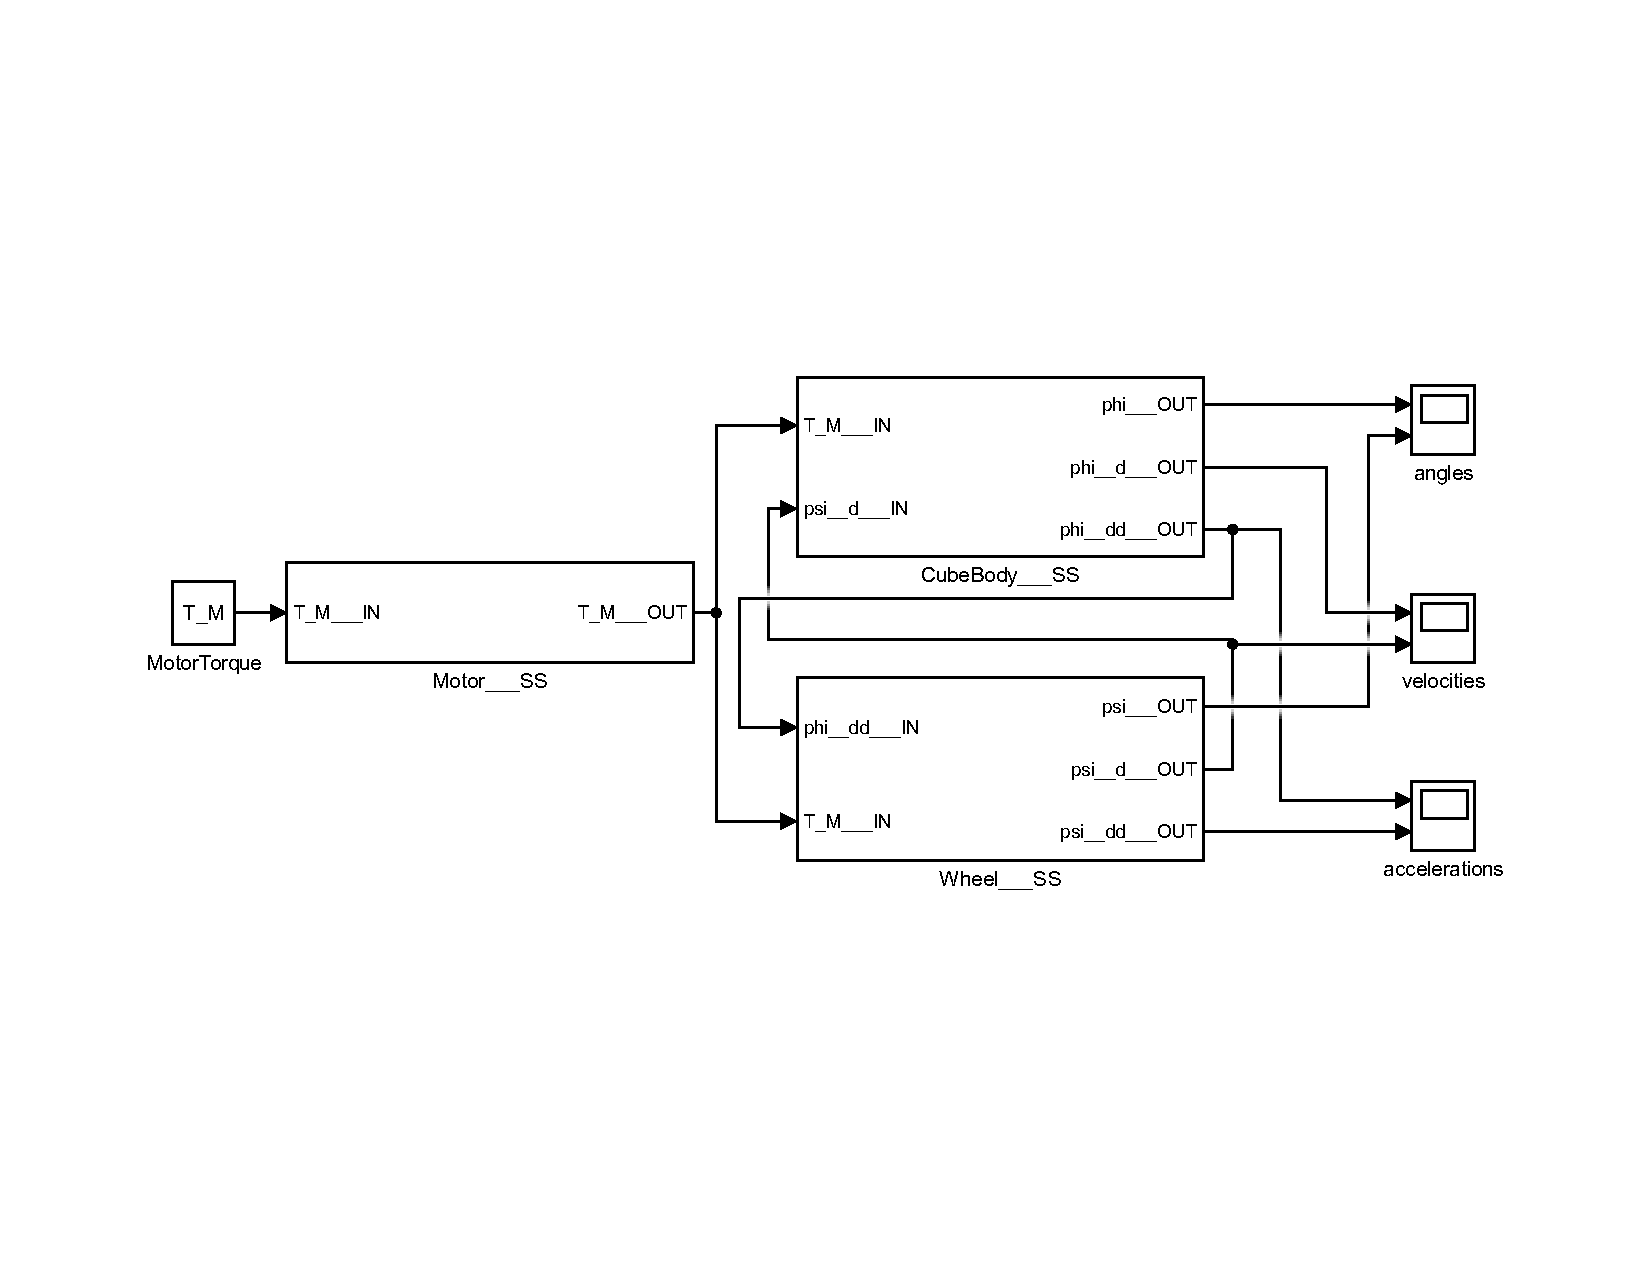
\includegraphics[width=\linewidth, trim={0 7cm 0 6cm},clip]{model_1D_overview}
\caption{Simulink-Modell Übersicht, Quelle: eigene Darstellung}
\end{figure}

\subsubsection{Simulation des Motors}
Der Motor wird als zwei in Reihe geschaltete PT1-Glieder simuliert. Da der Regler als Stellgröße ein Motormoment berechnet, beträgt die Verstärkung des Motor $K_M$ in der Simulation den Wert eins. Die Zeitkonstanten der PT1-Glieder sind einerseits die elektrische Zeitkonstante $T_e$ und die mechanische Zeitkonstante $T_m$, wessen Werte dem Datenblatt des Herstellers entnommen werden.

\begin{equation}
K_M = 1 \hspace{35pt} T_e = 0.55ms \hspace{35pt} T_m = 12.4ms
\end{equation}

\subsubsection{Simulation der Würfelseite}
Die Dynamik der Würfelseite wird von \ref{BG_phi_quation} beschrieben.

\begin{equation}
\ddot{\varphi} = \frac{g(m_R \cdot l_{AB}^2 + m_K \cdot l_{AC})sin(\varphi) - C_{\varphi} \cdot \dot{\varphi} + C_{\psi} \cdot \dot{\psi} - T_M}{{\theta}^A_K + m_R \cdot l_{AB}^2} \tag{\ref{BG_phi_quation}}
\end{equation}

Somit ist die Winkelbeschleunigung gleich der Summe der Drehmomente geteilt durch die betroffenen Massenträgheitsmomente. Durch Integration und Rückführung können die einzelnen Drehmomente berechnet werden. Das folgende Modell zeigt die Umsetzung dieser Berechnungsvorschrift in Simulink.

\begin{figure}[h]
\label{Simulink_1DModell_CubeBody_pic}
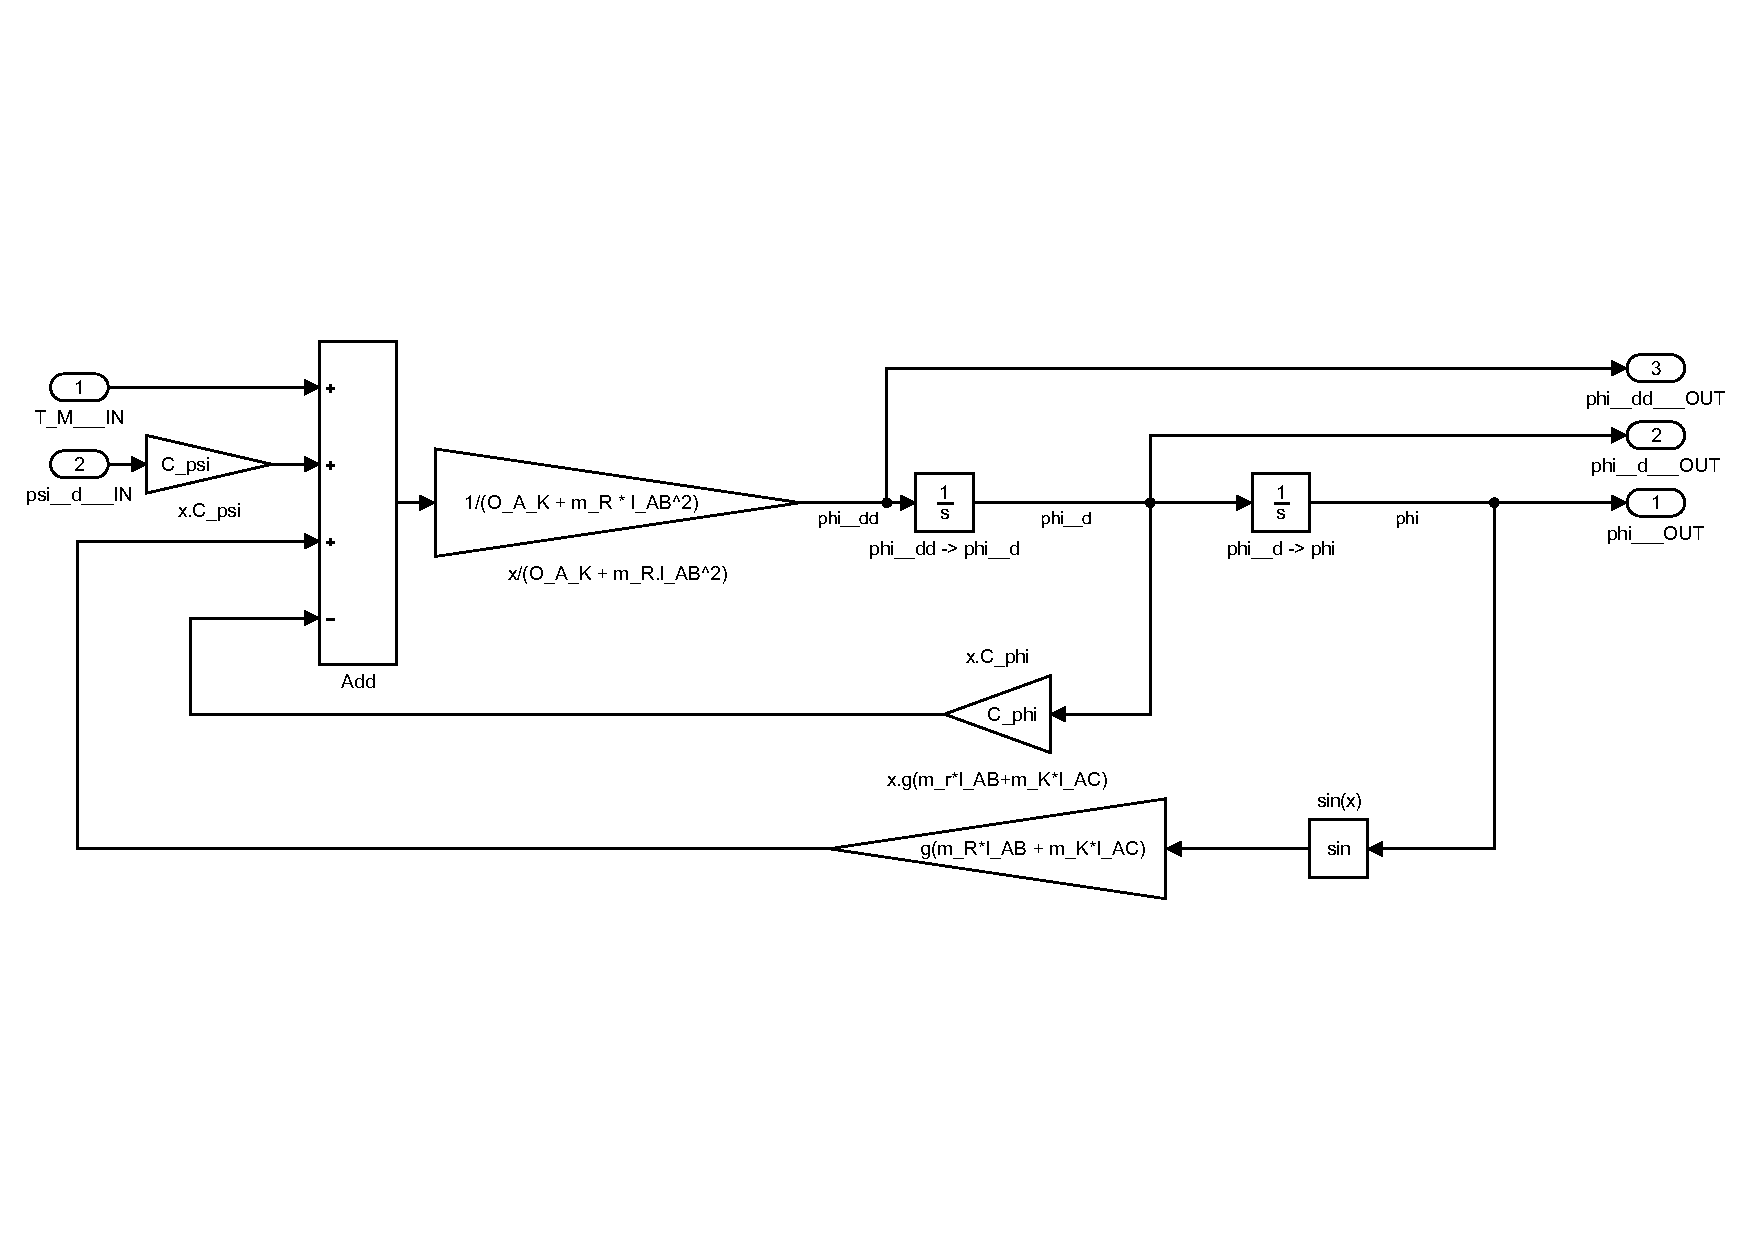
\includegraphics[width=\linewidth, trim={0 5cm 0 5cm},clip]{model_1D_cubebody}
\caption{Subsystem Würfelseite, Quelle: eigene Darstellung}
\end{figure}

\subsubsection{Simulation der Schwungmasse}
Die Dynamik der Schwungmasse wird von \ref{BG_psi_equation} beschrieben, allerdings wird das Modell vereinfacht indem $\ddot{phi}$ nicht substituiert wird.

\begin{equation}
{\theta}^R_B \cdot \ddot{\psi} = T_M - C_{\psi} \cdot \dot{\psi} - {\theta}^B_R \cdot \ddot{\varphi}\tag{\ref{BG_psi_equation}}
\end{equation}

Das Simulink-Modell folgt dem selben Schema wie das Subsystem zur Simulation der Bewegung des Würfelkörpers.

\begin{figure}[h]
\label{Simulink_1DModell_Wheel_pic}
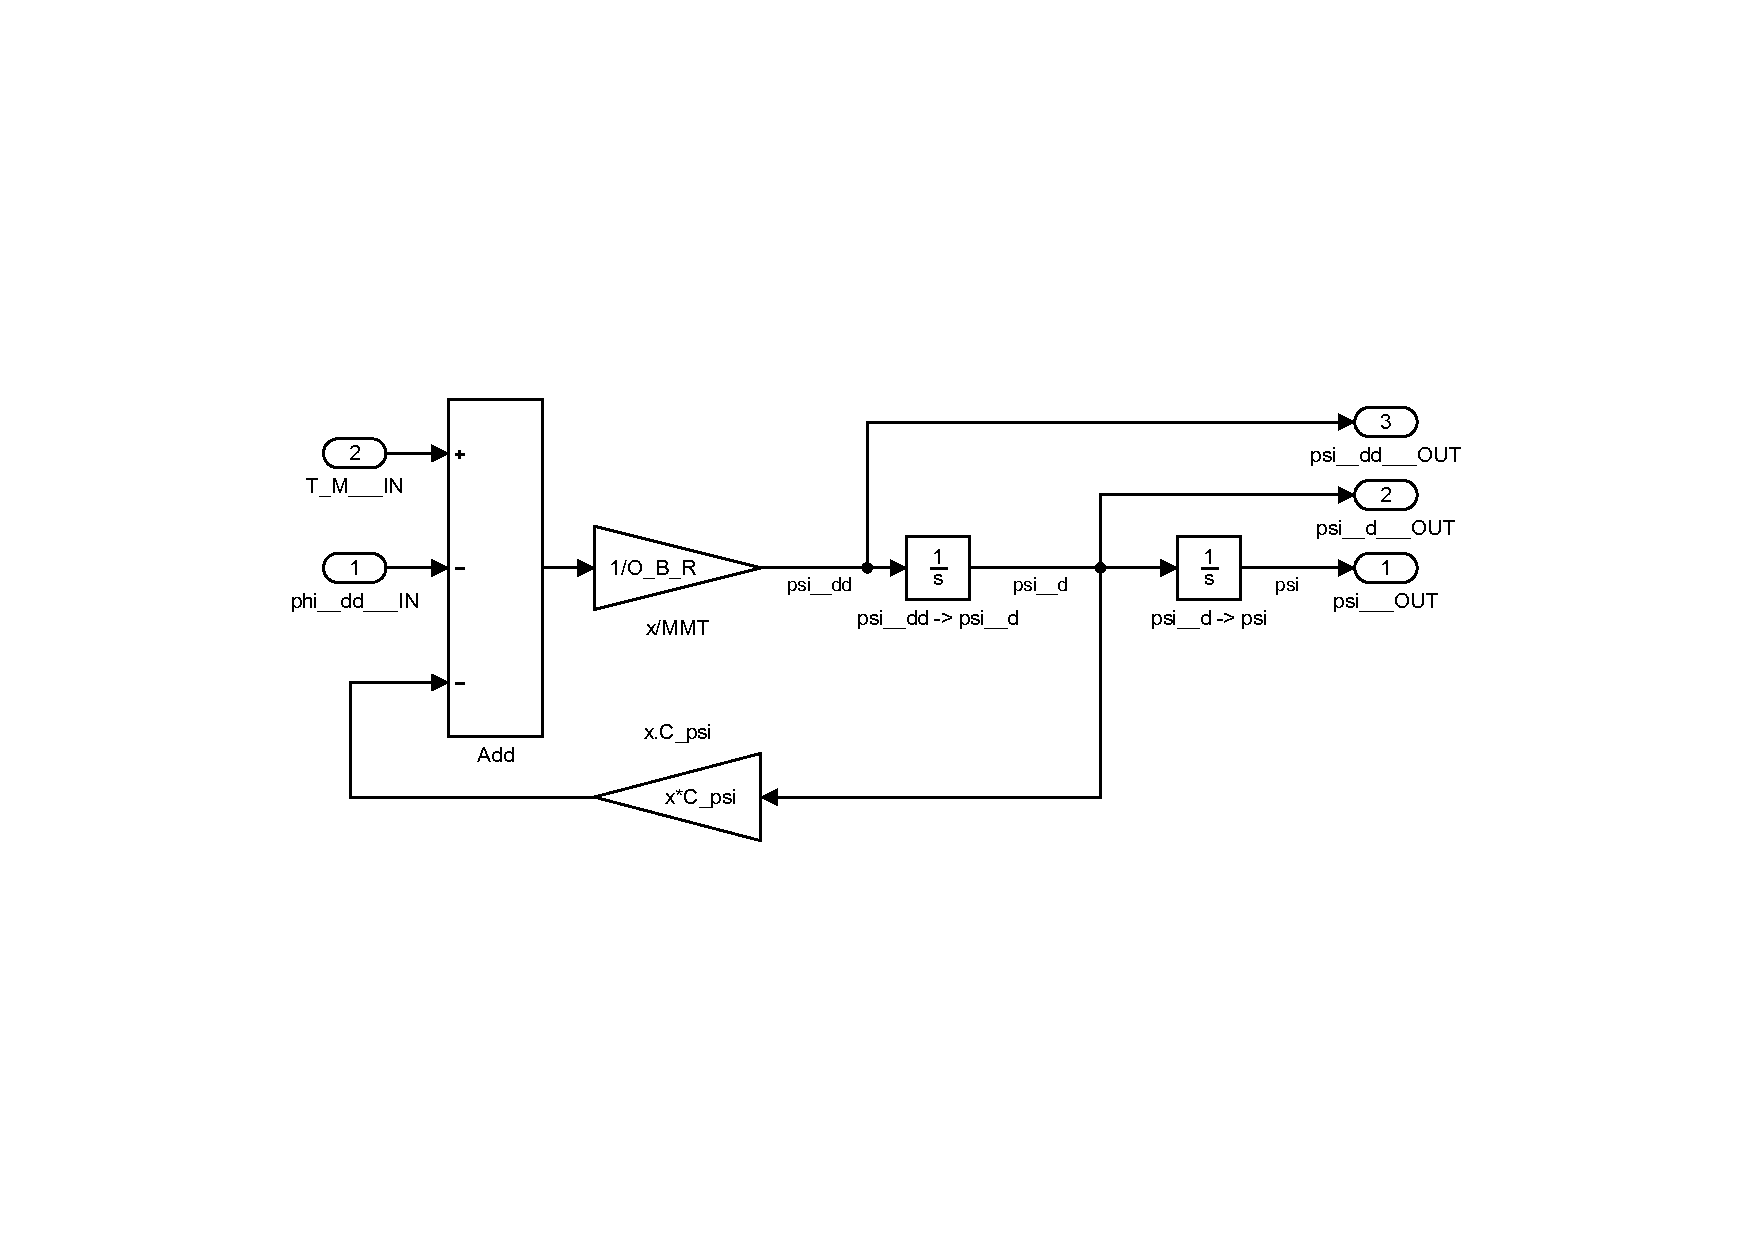
\includegraphics[width=\linewidth, trim={0 6cm 0 6cm},clip]{model_1D_wheel}
\caption{Subsystem Schwungmasse, Quelle: eigene Darstellung}
\end{figure}

\newpage
\begin{thebibliography}{\hspace{0.5cm}}
	\bibitem{TheoPhysik1} Wolfgang Nolting: Grundkurs Theoretische Physik 1 - Klassische Mechanik
	\bibitem{TheoPhysik2} Wolfgang Nolting: Grundkurs Theoretische Physik 2 - Analytische Mechanik
	\bibitem{Kane} Thomas R. Kane: Dynamics - Theory and Applications
	\bibitem{SuS} Ottmar Beucher: Signale und Systeme - Theorie, Simulation und Anwendung

\end{thebibliography}


\end{document}